% +++
% sequence = ["latex", "bibtex", "latex", "latex"]
% [programs.latex]
% 	command = "lualatex"
% 	opts = ["-synctex=1", "-file-line-error", "-interaction=nonstopmode"]
% 	args = ["%S"]
% [programs.bibtex]
% 	command = "upbibtex"
% 	target = "../ref.bib"
% 	args = ["%B"]
% +++

\documentclass[./main]{subfiles}
\graphicspath{{\subfix{./figures/section3/}}}
\setcounter{section}{2}

\begin{document}
\section{再三のコンパイルと自動化}
\addtocontents{lof}{\protect\addvspace{1em}}
\noindent
ここまで\verb|tex|ファイルから文書出力を得ることを曖昧に``処理''と表現してきた.
この``処理''とは実際にはどのような``処理''をおこなっているのかについて説明していく.
具体的には,\pdfTeX 系なのか否かや相互参照・文献情報の有無によって必要な処理の種類・順番や回数が変わる.
最近では\verb|latexmk|というコマンドのおかげで,このことを意識しなくてもいいことが多いが,この処理について知っておくことは\verb|latexmk|丸投げよりも効率がいい処理も可能で,デバッグの役にも立つので,知っておいて損はないと思う.
なお,\verb|latexmk|という名前からも分かる通り,今後の話は\LaTeX まわりの話である.

\subsection{texファイルからpdfファイルまで}
\noindent
まず\verb|latexmk|に丸投げして普段考えない,\verb|tex|ファイルから\verb|pdf|ファイルを出力するまでの処理の流れについて簡単に説明する\supercite{LaTeXcompile_Yamamoto}.
なお,以下では作成した\verb|tex|ファイルの名前を\verb|hoge.tex|とする.
ユーザは\verb|hoge.tex|の中身に従い,適切なマクロ体系を選択する.
というよりも,日本語を使うのか,Unicodeを使うのか,ユーザ好みのフォントを選びたいのか,といった目的に応じて選択すべきマクロ体系があり,それに合わせて\verb|hoge.tex|を作成する.
今後,例として\LuaLaTeX $+$\upBibTeX を用いることにする.


\subsubsection{はじめての\LaTeX コンパイル}\label{1stLaTeX}
\noindent
選択したマクロ体系で処理をする: 
\begin{center}
  \verb|lualatex hoge.tex|
\end{center}
これにより,次のファイルが生成される: 
\begin{itemize}
  \item 出力ファイル
  \begin{itemize}
    \item \verb|hoge.dvi|: \LaTeX, (u)\pLaTeX などを用いた場合
    \item \verb|hoge.pdf|: \pdfLaTeX, \XeLaTeX, \LuaLaTeX などを用いた場合
  \end{itemize}
  \item 補助ファイル\verb|hoge.aux|: 相互参照・ラベルの情報を保存する.
  \item ログファイル\verb|hoge.log|: コンパイル時の記録.エラーや警告も保存される.
\end{itemize}
このとき,もともと相互参照に関する\verb|hoge.aux|を読み込まずに\verb|hoge.tex|のコンパイルを行ったため,今回の出力で適切な相互参照はできていない.
相互参照されるべきところでは``??''が表示され,\verb|hoge.log|には参照が見つからなかった旨の警告\footnote{LaTeX Warning: There were undefined references.}が記録される.
これは一度の処理を高速・省メモリで終えるために,1回あたりのコンパイルでは\verb|tex|ファイルを最初から最後まで順に読み込みながら出力を行っているからである.
このコンパイルの最中に補助ファイル(\verb|hoge.aux|)にラベルを前から順に保存していく.

次のステップは文書の中に相互参照が含まれるかどうかによって以下のように場合分けされる: 
\begin{table}[ht]
  \centering\begin{tabular}{ll}\bhline{1.5pt}
     & 次の処理 \\\hline
    参照したい文献\verb|\cite|がある場合 & \ref{BibTeX}参考文献処理\\
    参考文献以外の相互参照\verb|\ref|のみある場合 & \ref{2ndLaTeX}相互参照を処理する\LaTeX コンパイル\\
    相互参照も参考文献もない場合 & \ref{dvipdfmx} 文書のpdf出力を得る \\\hline
  \end{tabular}
\end{table}

\subsubsection{参考文献処理}\label{BibTeX}
\noindent
所望の形に整形された参考文献の一覧を作る: 
\begin{center}
  \verb|upbibtex hoge.aux|
\end{center}
具体的には,\ref{1stLaTeX}はじめての\LaTeX コンパイル\ によって\verb|hoge.aux|ファイル内に保存された文献リストの雛形から所望の形の文献リストが\verb|hoge.bbl|に生成される\supercite{参考文献_星野}.
これは,\verb|thebibliography|環境であり,\BibTeX 等を使わずに手動で\verb|\bibitem|などとちまちま書いていくアレである.
つまり,\verb|hoge.bbl|にはそれぞれの情報を含めた文献項目(\verb|bibitem|とか\verb|entry|)が所望の形式で出力できるように収められている.

次のステップは\ref{2ndLaTeX}文献リストを出力する\LaTeX コンパイル.

\subsubsection{文献リストを出力する\LaTeX コンパイル}\label{2ndLaTeX}
\noindent
\verb|hoge.bbl|を使って,文献リストを出力しつつ,補助ファイル\verb|hoge.aux|に文献に関わる相互参照情報を保存する.
\begin{center}
  \verb|lualatex hoge.tex|
\end{center}
ちなみに,\ref{1stLaTeX}で作られた相互参照は今回の\LaTeX コンパイル時に読み込まれた\verb|hoge.aux|を使って,解決される.
なぜならこのコンパイル時にはすでに1回目のコンパイルで作成された\verb|hoge.aux|があり,そこに文献参照以外の必要な相互参照の情報が保存されているからである.

次のステップは\ref{3rdLaTeX}相互参照を処理する\LaTeX コンパイル.

\subsubsection{相互参照を処理する\LaTeX コンパイル}\label{3rdLaTeX}
\noindent
\verb|hoge.aux|の相互参照を解決し,\verb|hoge.dvi|か\verb|hoge.pdf|を出力する: 
\begin{center}
  \verb|lualatex hoge.tex|
\end{center}
補助\verb|aux|ファイルの中に前回保存したラベルがあるため,その番号を採用・出力していく.
御存知の通り,出力が\verb|dvi|ファイルになるか\verb|pdf|ファイルになるかはマクロ体系として何を使うかに依存する.
直接\verb|pdf|ファイルが出力される系統を用いているのであれば,ここで文書は完成である.
\begin{table}[ht]
  \centering\begin{tabular}{lcc}\bhline{1.5pt}
    マクロ体系 & 出力 & 次の処理 \\\hline
    \LaTeX, (u)\pLaTeX & \verb|hoge.dvi| & \ref{dvipdfmx}文書のpdf出力を得る\\
    \pdfLaTeX, \XeLaTeX, \LuaLaTeX & \verb|hoge.pdf| & -\\\hline
  \end{tabular}
\end{table}

\subsubsection{文書のpdf出力を得る}\label{dvipdfmx}
\noindent
すでに述べたが,\verb|dvi|ファイルとは DeVice-Independent file のことで,文書の見た目のレイアウトを画像形式・表示デバイス・プリンタなどにまったく依存しない形で記録している\supercite{DVI_Wikipedia}.
これは人間が読むように設計されておらず,DVIドライバと呼ばれる別のプログラムに入力することで,画像として表示したり,文書形式に変換したりできる.
主なDVIドライバとしては次のようなものがある: 
\begin{itemize}
  \item \verb|dvipdfmx|: \verb|dvi|\textrightarrow \verb|pdf|.日本語文書作成においては最もよく使われている.そもそも海外では\pdfLaTeX とその周辺が主流であり,\verb|dvi|ファイルは生成されないのである.
  \item \verb|dvips|: \verb|dvi|\textrightarrow \verb|ps| (PostScript).この\verb|ps|ファイルとは\verb|pdf|ファイルの基礎となったものである\supercite{PostScript_Wikipedia}.
  \item \verb|dviout|: (u)\pTeX 対応のDVIプレビューア.最近では推奨されない.
\end{itemize}

\subsubsection*{特別なスープ}
\noindent
文書作成の具体的な流れはここまでで説明したとおりである.
基本的な相互参照にしろ,文献の参照にしろ,ラベルを適切に補助\verb|aux|ファイルに保存できれば,その後もう一回コンパイルすることですべての参照がきちんと対応して出力される.
つまり,文献参照が必要ない(もしくは\verb|bbl|ファイルに変更がない)場合には2回のコンパイルによって出力が得られることになる.
これは基本的に間違ってはいないが,実際には2回では済まない場合がある.
具体的には,参照したいラベル先が不明でとりあえず``??''と出力されていた部分に,ラベルがついている数字や文献を表す記号などが正しく代入されることで改ページの場所や図表の位置が変わってしまった場合,ラベルと番号の対応付けが変わってしまい,参照番号が正しく振られていないことになってしまうことがある\footnote{LaTeX Warning: Label(s) may have changed. Rerun to get cross-references right.}.
そこで次のような収束しないおもちゃを作ることができる\supercite{loop_Qiita}: 
\begin{lstlisting}
\documentclass{article}
\pagenumbering{roman}
\setlength{\textwidth}{5em}
\setlength{\textheight}{2\baselineskip}
\begin{document}
  \setcounter{page}{999}
  \noindent The Page Number \pageref{foo} is\label{foo} shaking up and down.
\end{document}
\end{lstlisting}
この\TeX 文書をコンパイルした結果を\figref{fig:loop}に示す.
$n\in\mathbb{Z}_{+}$回コンパイルしたあとの出力において,ラベルが付けられる``is直後''のページ番号とそれを参照しているはずの\verb|\pageref{foo}|の出力は必ず一致しない.
このおもちゃに面白い以上の意味は見いだせないが,これが理解できれば,相互参照のために\verb|aux|ファイルが必要で,同様に複数回のコンパイルが必要なこともわかるであろう.
\begin{table}[h]
  \centering\begin{tabular}{ccc}\bhline{1.5pt}
    number of compile & page no. which contains \verb|\label| & output of \verb|\pageref| \\ \hline
    1 & 999(cmxcix) &?? \\
    even &1000(m)& cmxcix \\
    odd & 999(cmxcix) & m \\\hline
  \end{tabular}
\end{table}
\begin{figure}[h]
  \centering
  \begin{tabular}{|c|c|c|}\hline
    &former&latter\\\hline
    odd&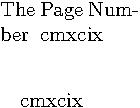
\includegraphics[scale=1]{odd.pdf}
    &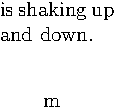
\includegraphics[scale=1]{odd2.pdf}\\\hline
    even&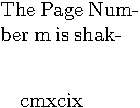
\includegraphics[scale=1]{even.pdf}
    &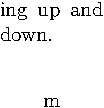
\includegraphics[scale=1]{even2.pdf}\\\hline
  \end{tabular}
  \caption{Example of not converging cross-referencing. Upper: former (left) and latter (right) page of the output pdf file after odd times compile. Lower: output after even times compile.}
  \label{fig:loop}
\end{figure}

\subsection{自動化}
\noindent
ここまででわかるように,文献を含む相互参照をきちんと機能させるためには,補助ファイル\verb|hoge.aux|の存在も,それを使って複数回コンパイルすることも必要不可欠である.
一方で,そのコンパイル回数はある程度目処がつくとは言え,正確に予測することは困難である.
このような状況で,変更のたびに参照が失敗している箇所がないか確認しながら自分の手でコンパイルしていくのは大変面倒である.

この「複数回コンパイル等に起因する煩雑さ」を解決・軽減する方法として有名なのはもちろん
\begin{itemize}
  \item \verb|latexmk|: 現在最も有名な自動化ツール  \footnote{個人的にはlatexmkが広く使われる理由として「煩雑な操作に対して特別何も考えなくてもいつでもどこでも大体なんとなくうまくいく」ことが挙げられると思っている.しかしだからこそ冗長性を持ち,無駄が多いのではないかと感じる部分もある.}.
  複数回の実行に加え,\BibTeX 等の関連ツールの実行も自動で行える.
  \verb|latexmk|は\verb|aux|ファイルの内容が変化したときにコンパイルし直すことになっている.
  例えば\verb|aux|ファイルに時刻の情報を含むようなコードを書けば,コンパイルのたびに\verb|aux|ファイルが変化することになる\footnote{latexmkでは上限回数が設定されており,これにより無限の彼方に飛ばされることはない\supercite{TeXあれこれ_雑記帳}.}.
\end{itemize}
であるが,オリジナルの\TeX の拡張が様々存在することや,\TeX を使いやすくするためのマクロ体系も何種類も存在したことなどを考えれば,この自動化ツールが何種類も存在することは至極自然なことに感じられる.
いくつかのコンパイルツールを下記に示すが,「煩雑だな」と感じるのは同じでもそれを解消するための設計指針や思想は異なっているものも多い.
\begin{itemize}
  \item \verb|latexn|: 
  \item \verb|ptex2pdf|: \verb|(u)platex| と\verb|dvipdfmx|をまとめて実行する.
  \item \verb|llmk|: Light Latex MaKe.
\end{itemize}


\ifSubfilesClassLoaded{%
  \printbibliography
}% 

\end{document}
